\documentclass[11pt]{article}
\usepackage[margin=1in]{geometry}
\usepackage[T1]{fontenc}
\usepackage{lmodern,graphicx,booktabs,amsmath,hyperref,caption,float,microtype,xcolor,array,enumitem}
\graphicspath{{../figures/}}
\hypersetup{colorlinks=true,linkcolor=blue!50!black,urlcolor=blue!50!black,citecolor=blue!50!black}
\captionsetup{font=small,labelfont=bf,skip=4pt}
\setlength{\parskip}{4pt}
\renewcommand{\arraystretch}{1.12}
\title{\textbf{Counting the Ones That Got Away:\\ A Measurement Study of Missed Interception Chances\\ in the NFL, 1999--2026}}
\author{Nikhil Chandrashaker}
\date{Working draft, November 2026}
\begin{document}
\maketitle

\begin{abstract}\noindent
Defenders who drop catchable interceptions are not tracked in any official NFL statistic. The idea of counting them is at least as old as a 2009 fan proposal, and a commercial vendor charts them behind a paywall, but no open data set exists. We build two. For 2022--2026 we combine nflverse play-by-play, FTN charting and rosters to define a \emph{missed-INT chance} (MIC): a throw charted as interception-worthy that fell incomplete while a defensive back or linebacker was credited with the pass defense. Of 2,841 interception-worthy throws in 2022--2025, 49\% were intercepted and 30\% became MIC. Because FTN charting starts in 2022, we add a long-run companion for 1999--2026 built from play-by-play alone: interceptions against other passes defended (PD). Conversion differs sharply by position (charted: safeties 73\%, cornerbacks 62\%, linebackers 54\%). In the four charted seasons, conversion within a position cannot be told apart from luck (split-half $r$ = 0.08, 95\% CI -0.05 to 0.20). The 27-season long-run data do detect a small stable component (year-to-year $r$ = 0.16), which needs roughly 22 to 46 chances to reach half reliability. Chances (INT plus misses) predict next-season interceptions better than interceptions alone, in 22 of 26 held-out seasons, and an extra pass defended carries about 0.45 times the predictive weight of a pick (a charted missed chance about 0.7 times). Over the same period the interception rate fell by about 30\%. We conclude that an official statistic should report \emph{chances} and a shrunk, position-adjusted conversion rate; a bare drop count would mostly rank defenders by noise.
\end{abstract}

\section{Introduction}
Interceptions are the most valued event a pass defender produces, yet the box score credits only the ones that were caught. A defender who gets both hands on a throw and lets it fall is recorded the same way as one who was beaten. Swartz \cite{swartz2009} proposed in 2009 that the NFL record each dropped interception and divide interceptions by interceptions plus drops to measure a defender's hands. Pro Football Focus (PFF) charts such drops and has published leaderboards, for example reporting that one cornerback led the league with 15 dropped interceptions from 2020 and that a safety had dropped one of 13 chances over the same stretch \cite{pff2024}. The underlying player-level data are behind a subscription, and the NFL does not publish them.

This paper asks three questions that matter for deciding whether a dropped-interception statistic deserves official status.
\begin{enumerate}[nosep]
\item \textbf{Can it be measured openly?} We construct a proxy from public data and document its error.
\item \textbf{Is it a skill?} We test whether a defender's rate of converting chances is stable and distinguishable from chance.
\item \textbf{Is it useful?} We test whether counting misses improves prediction of future interceptions at the player and team level.
\end{enumerate}
Our contributions are a reproducible data set (events, player-seasons, team-seasons, and a charting-quality audit), an interactive dashboard, a long-run companion measure covering 1999--2026 that lets us ask the same questions of 27 seasons, and a set of estimates that bound how much any missed-interception statistic can tell us at NFL sample sizes.

\section{Data}
\textbf{Sources.} We use nflverse play-by-play for 2022 through Week 9 of 2026 \cite{nflverse}, FTN charting data distributed through nflverse \cite{ftn}, and nflverse rosters. FTN charters flag each throw as \texttt{is\_interception\_worthy}, a charter's judgment that the throw could reasonably have been intercepted. FTN coverage of pass plays is at least 99.6\% in every season. Position comes from each roster's depth-chart position, which separates CB, FS, SS, ILB, MLB and OLB where the coarse position field says only ``DB'' or ``LB''.

\textbf{Scope.} We keep pass attempts that are not sacks or spikes. Player-season tables use the regular season only (2,669 event credits); the event file also carries postseason plays. Partial 2026 data are flagged. They are excluded from the empirical-Bayes priors, the prediction models and the team persistence tests, which use four complete seasons (2022--2025), and are included in career totals, the funnel plots and the split-half test.

\textbf{Long-run extension.} FTN charting begins in 2022, so MIC cannot be built for earlier years. For 1999 through Week 9 of 2026 we use play-by-play and rosters only: 58,303 credits to defensive backs and linebackers (regular season and postseason), of which 12,990 are interceptions and 45,313 are passes defended. Defender identifiers are present on every interception in every season, and credited pass defenses run at roughly 9 to 12 percent of attempts without a break, so the credit data are consistent across eras. Positions come from the depth chart where present and from the roster position otherwise; defenders listed only as ``DB'' account for 11\% of chances in 1999--2001 and 2\% overall, and form their own group in the data. Defensive linemen are excluded (13\% of credits).

\begin{figure}[H]\centering
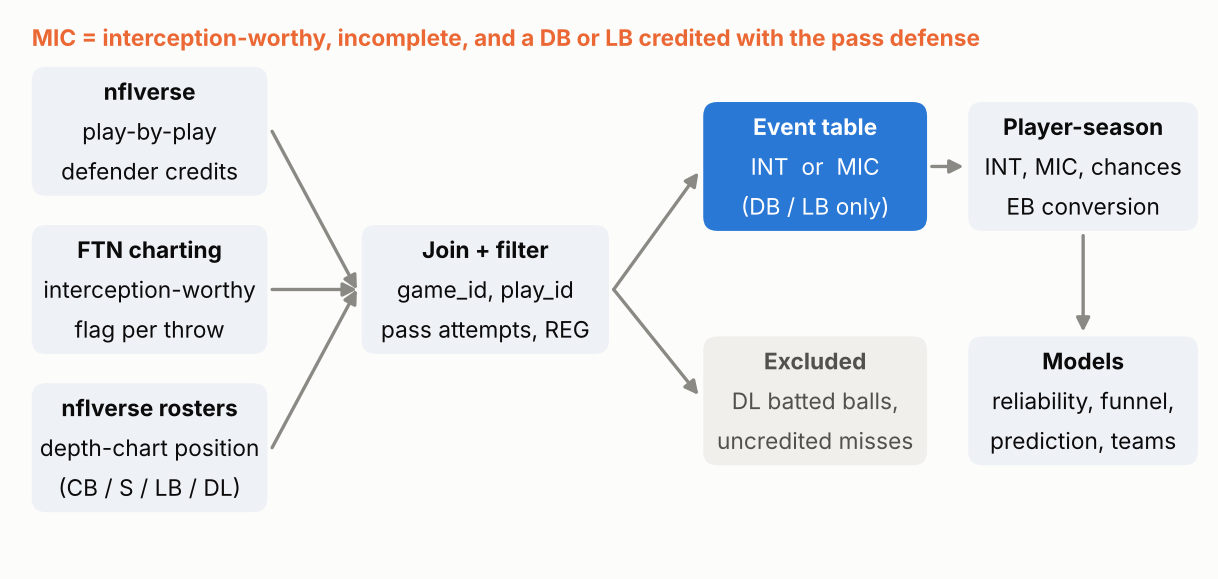
\includegraphics[width=\linewidth]{fig0_pipeline.png}
\caption{Data pipeline. Three open sources are joined at the play level and reduced to a table of INT and MIC credits for defensive backs and linebackers.}
\end{figure}

\section{Definitions and measurement}
\textbf{Interception (INT).} An interception credited to a defender in play-by-play.

\textbf{Missed-INT chance (MIC).} A pass attempt that FTN flagged interception-worthy, that was not intercepted, that was incomplete, and on which a defensive back or linebacker is credited with the pass defense (either of the two pass-defense slots). One credit is counted per credited defender.

From these we define, for a defender or team,
\begin{equation}
\text{Chances}=\text{INT}+\text{MIC},\qquad
\text{Convert}=\frac{\text{INT}}{\text{Chances}},\qquad
\text{MIC rate}=1-\text{Convert}.
\end{equation}
Convert is the quantity Swartz proposed (interceptions divided by interceptions plus drops), with MIC standing in for drops.

\textbf{Passes defended and INT share (long-run).} PD is a pass defense credited to a defensive back or linebacker on an incomplete pass that was not intercepted, with one credit per credited defender. The long-run analogue of Convert is
\begin{equation}
\text{INT share}=\frac{\text{INT}}{\text{INT}+\text{PD}}.
\end{equation}
PD makes no judgment about catchability, so most PD were never chances: INT share averages 22\%, against 64\% for charted conversion. We use it for relative questions (position, era, persistence, prediction) and validate it against MIC in Section~\ref{sec:val}.

\textbf{Why MIC is a proxy.} A true drop requires a judgment that the defender had the ball in his hands or a clean opportunity. MIC records a weaker thing: the defender touched a throw that was dangerous. That includes legitimate break-ups of passes the receiver also contested, so MIC overstates drops. It also omits drops by defenders who are not credited with a pass defense when they fail to catch the ball, so it can understate them. We treat MIC as an upper bound and test whether conclusions survive that error in Section 6. Figure~\ref{fig:funnel} shows where interception-worthy throws end up.

\begin{figure}[H]\centering
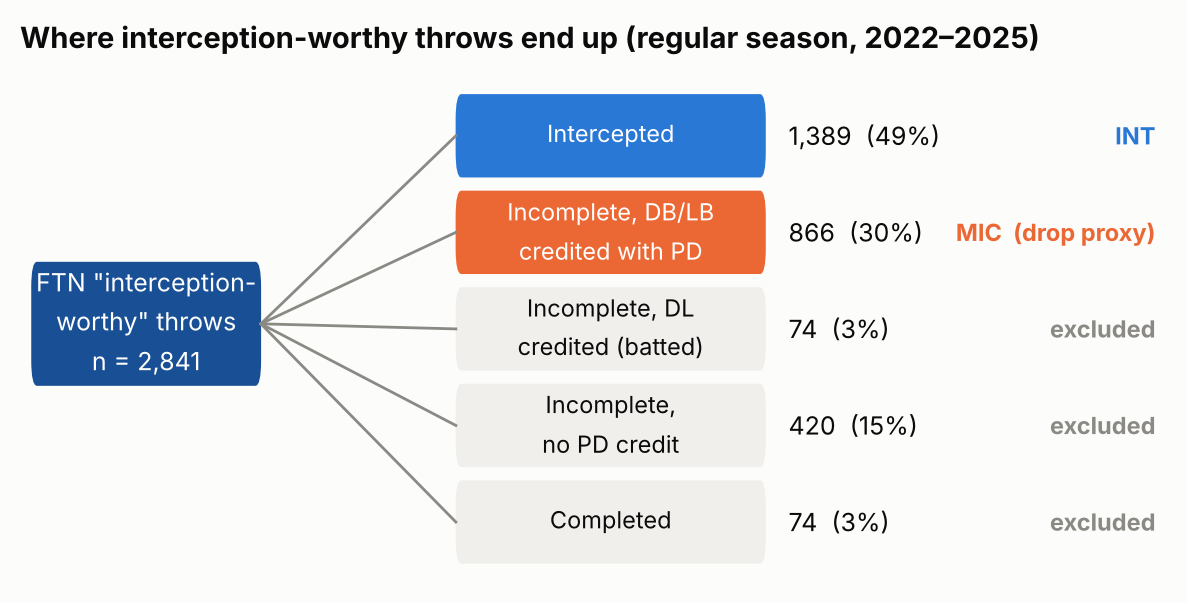
\includegraphics[width=0.92\linewidth]{fig1_funnel.png}
\caption{Outcomes of FTN interception-worthy throws, regular season 2022--2025. Percentages are shares of all interception-worthy throws; MIC counts plays, so it is slightly smaller than the MIC credit count when two defenders share a pass defense.}
\label{fig:funnel}
\end{figure}

\textbf{Charting drift.} The charted rate fell by about 38\% between 2022 and 2025 (Figure~\ref{fig:drift}), while actual interception rates were flat. We read this as a change in how FTN applies the flag, not in football. All cross-season comparisons below use rates, hold out whole seasons, or both, and counts are never compared across seasons without that caveat.

\begin{figure}[H]\centering
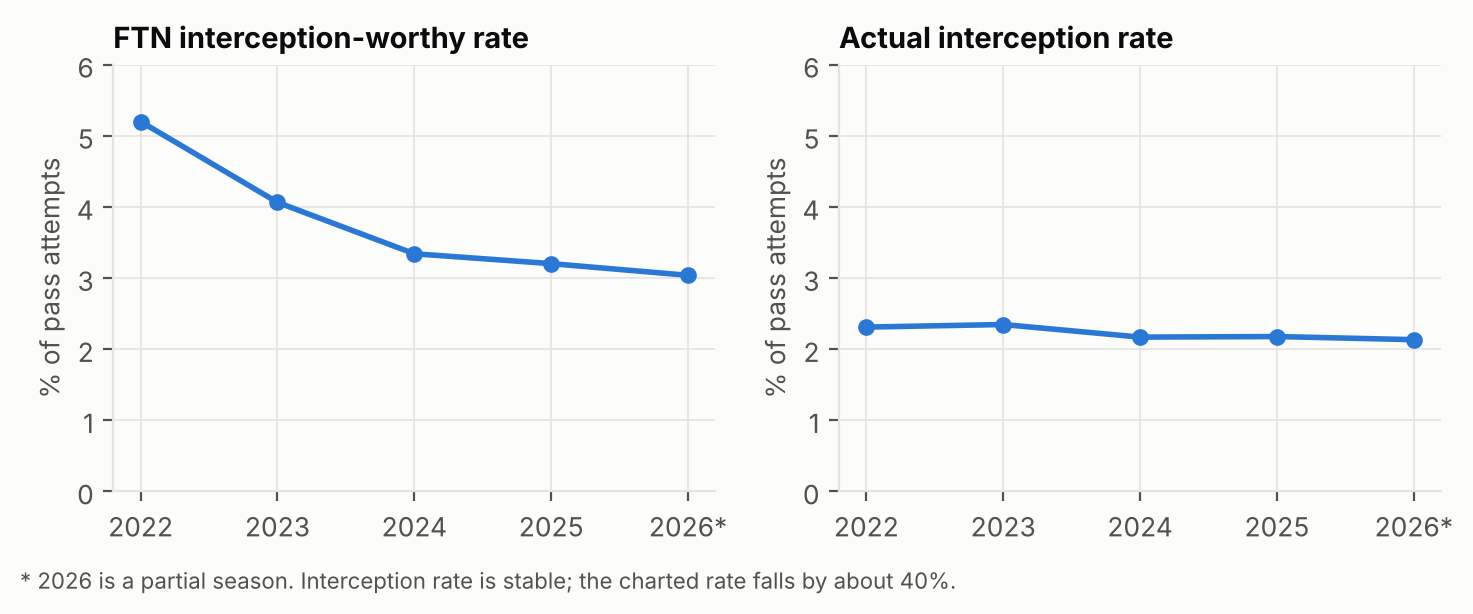
\includegraphics[width=0.95\linewidth]{fig2_drift.png}
\caption{FTN's interception-worthy rate drops sharply across seasons while the interception rate does not.}
\label{fig:drift}
\end{figure}

\section{Methods}
\textbf{Empirical-Bayes conversion.} For each position group $g$ we model a defender's INT count in $n$ chances as Binomial$(n,p)$ with $p\sim\text{Beta}(\alpha_g,\beta_g)$ and fit $(\alpha_g,\beta_g)$ by maximum likelihood on complete player-seasons \cite{efronmorris1975}. The posterior mean $(\alpha_g+k)/(\alpha_g+\beta_g+n)$ is the \emph{shrunk} conversion rate. The prior strength $\alpha_g+\beta_g$ is the number of chances at which half of the variation in an observed rate is signal. We test the Beta-Binomial against a pure Binomial with a likelihood-ratio statistic, using the half-chi-square reference appropriate to a boundary hypothesis.

\textbf{Split-half reliability.} For every defender we assign each chance to the odd or even weeks of the regular season, compute conversion in each half, and correlate the two halves across defenders with at least 4, 6 or 8 chances. Confidence intervals use 1,000 bootstrap resamples of defenders. If conversion were a stable skill the correlation would be positive; under pure luck it is zero.

\textbf{Funnel plots.} Following Spiegelhalter \cite{spiegelhalter2005} we plot each defender's conversion against his number of chances with exact binomial 95\% and 99.8\% limits around the position mean. Under luck about 5\% of defenders fall outside the 95\% limits.

\textbf{Prediction.} For every defender with chances in season $t$ who is on a roster in $t{+}1$ we model next-season INTs with Poisson regression on position and last-season counts, using leave-one-season-pair-out cross-validation over 2022$\to$2023, 2023$\to$2024 and 2024$\to$2025 ($n=824$). We compare four models: position only; last-year INT; last-year Chances; and INT and MIC with separate coefficients. Coefficient uncertainty comes from 400 player-cluster bootstrap resamples. At team level we correlate season-$t$ totals with season-$(t{+}1)$ INTs over 96 team-season pairs.

\textbf{Long-run analyses.} The same estimators are applied to the 10,477 complete 1999--2025 cornerback, safety and linebacker player-seasons with INT and PD. Split-half and year-to-year correlations use residuals from each season-and-position league rate, so era shifts cannot create spurious correlation. Prediction uses leave-one-season-pair-out cross-validation over 26 pairs, with each count rescaled by the ratio of the sample-average league total to that season's league total. Team persistence is computed after subtracting each season's league mean. Bootstrap intervals use 500 resamples (200 for the Poisson coefficients).

\section{Results}
\subsection{Conversion differs by position}
Figure~\ref{fig:pos} and Table~\ref{tab:pos} show that the share of chances converted is far from uniform. Safeties catch about three in four, cornerbacks about three in five, and linebackers a little over half. The safety interval is clear of the other two, and the cornerback and linebacker intervals only just touch. A single league-wide benchmark would therefore be wrong for every position, and comparisons between defenders have to be made within position.

\begin{figure}[H]\centering
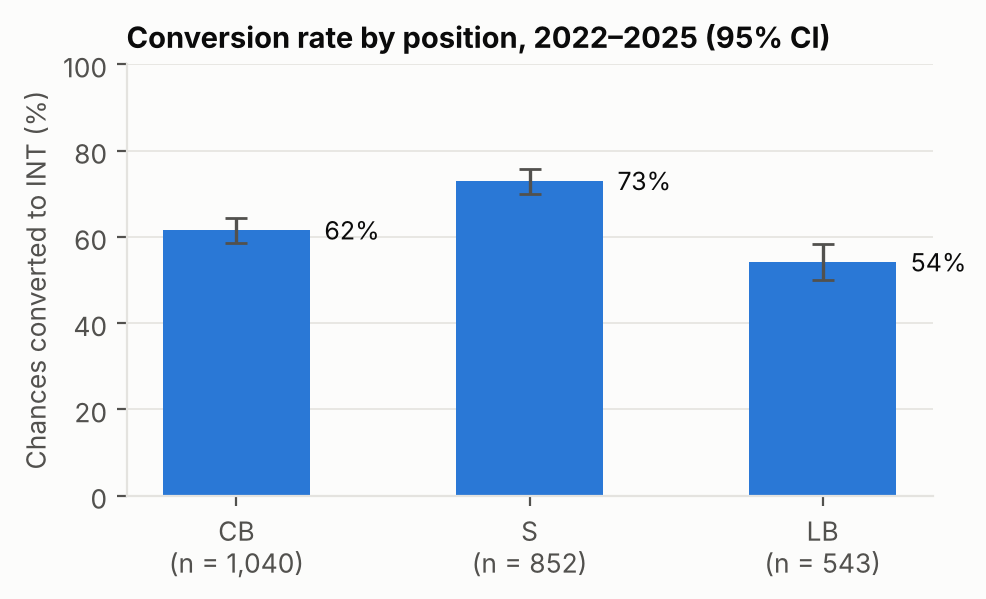
\includegraphics[width=0.62\linewidth]{fig3_position.png}
\caption{Conversion by position group, complete seasons 2022--2025, with 95\% Wilson intervals.}
\label{fig:pos}
\end{figure}

\begin{table}[H]\centering\small
\caption{Conversion by position group, complete seasons 2022--2025.}\label{tab:pos}
\begin{tabular}{lrrrrr}\toprule
Position & INT & MIC & Chances & Convert & 95\% CI \\ \midrule
S & 622 & 230 & 852 & 73\% & 70--76\% \\
CB & 640 & 400 & 1040 & 62\% & 59--64\% \\
LB & 294 & 249 & 543 & 54\% & 50--58\% \\
\bottomrule\end{tabular}\end{table}

\subsection{Is conversion a skill?}
\textbf{Reliability.} The fitted priors are tight: prior strength is 22 chances for cornerbacks, 27 for safeties and 63 for linebackers (Table~\ref{tab:over}). The median defender-season contains only 2 chances and 46\% of defender-seasons contain exactly one. At two chances only about 8\% of the variation in a cornerback's observed rate is signal (Figure~\ref{fig:rel}); a cornerback would need roughly 11 seasons at the median rate to reach 50\% reliability.

\begin{table}[H]\centering\small
\caption{Beta-Binomial fits and overdispersion tests by position group (complete player-seasons).}\label{tab:over}
\begin{tabular}{lrrrrr}\toprule
Position & Player-seasons & $\alpha+\beta$ & True-talent SD & LRT & $p$ \\ \midrule
CB & 461 & 22.3 & 10.1 pts & 1.85 & 0.09 \\
S & 352 & 27.5 & 8.3 pts & 1.08 & 0.15 \\
LB & 316 & 63.0 & 6.2 pts & 0.09 & 0.38 \\
\bottomrule\end{tabular}\end{table}

\begin{figure}[H]\centering
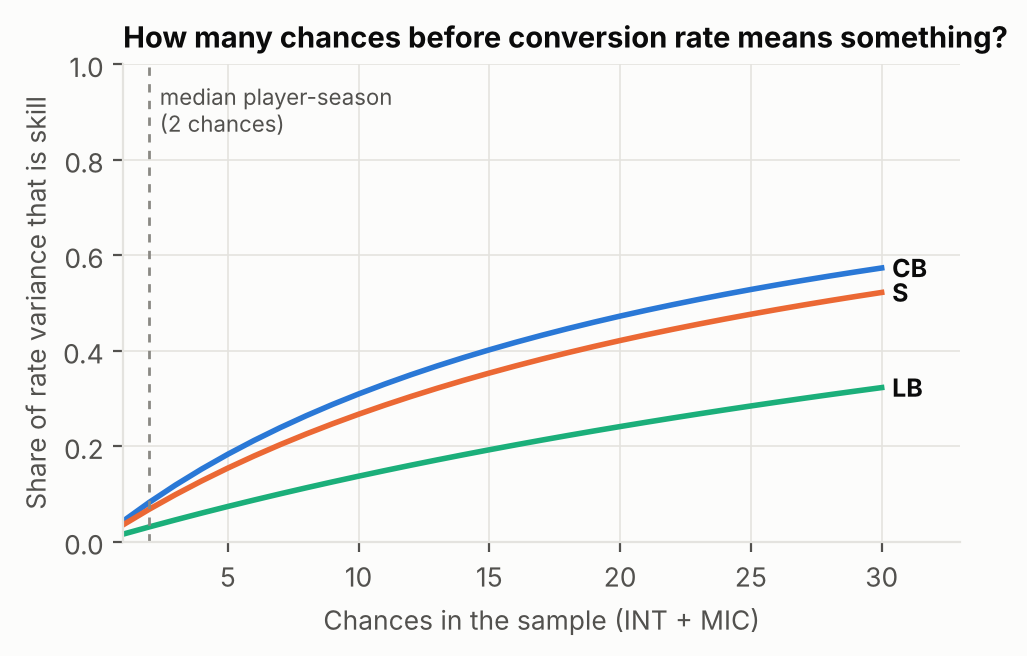
\includegraphics[width=0.72\linewidth]{fig4_reliability.png}
\caption{Reliability of an observed conversion rate as a function of chances, $n/(n+\alpha+\beta)$.}
\label{fig:rel}
\end{figure}

\textbf{Overdispersion.} If defenders differed in true conversion skill, observed rates would vary more than binomial noise allows. The Beta-Binomial improves on the Binomial only weakly (Table~\ref{tab:over}); none of the three position groups rejects pure binomial variation at the 5\% level. The fitted true-talent standard deviation is about 6--10 percentage points depending on position, compared with a binomial standard error of about 35 points at two chances.

\textbf{Split-half.} Table~\ref{tab:split} shows split-half correlations that are indistinguishable from zero at every threshold. This is a finding about four seasons; Section~\ref{sec:long} repeats the test on 27. With six or more chances the correlation is 0.08 and the interval excludes only large values.

\begin{table}[H]\centering\small
\caption{Split-half (odd vs even weeks) correlation of conversion rate.}\label{tab:split}
\begin{tabular}{lrrrr}\toprule
Min. chances & Defenders & $r$ & 95\% CI & Spearman--Brown \\ \midrule
4 & 253 & -0.02 & -0.13 to 0.10 & -0.04 \\
6 & 169 & 0.08 & -0.05 to 0.20 & 0.15 \\
8 & 113 & 0.08 & -0.08 to 0.24 & 0.16 \\
\bottomrule\end{tabular}\end{table}

\textbf{Funnel plots.} Only 2 of 610 defenders sit outside the 95\% limits (Marlon Humphrey and Sauce Gardner), fewer than the roughly 5\% expected under luck; discrete outcomes make the nominal 95\% limits conservative, so this is consistent with luck rather than evidence for it. Figure~\ref{fig:funnelplot} shows the spread.

\begin{figure}[H]\centering
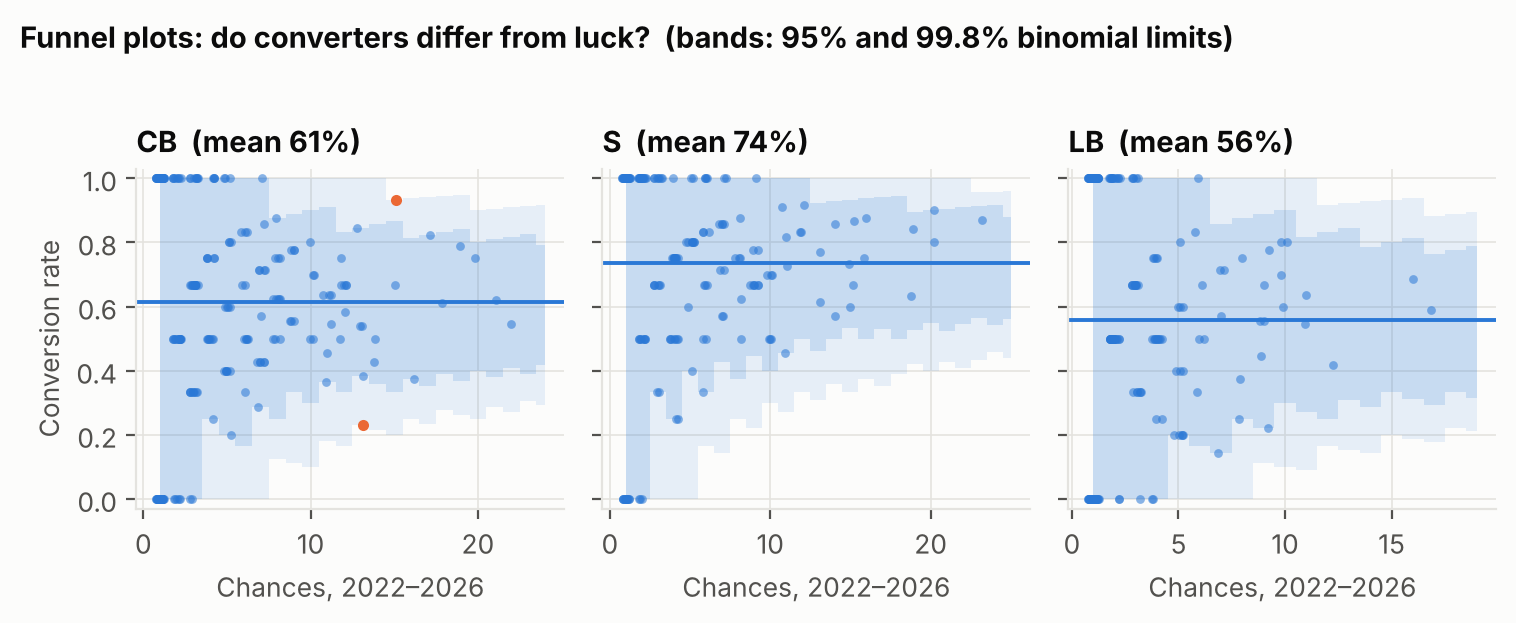
\includegraphics[width=\linewidth]{fig5_funnelplot.png}
\caption{Funnel plots by position, career totals 2022--2026. Orange points lie outside the 95\% limits.}
\label{fig:funnelplot}
\end{figure}

\textbf{Shrinkage.} Among the 71 defenders with at least ten chances, shrinkage reduces the standard deviation of conversion from 15 to 8 points (Figure~\ref{fig:shrink}). The dispersion that remains is dominated by position differences, which the position-specific priors retain.

\begin{figure}[H]\centering
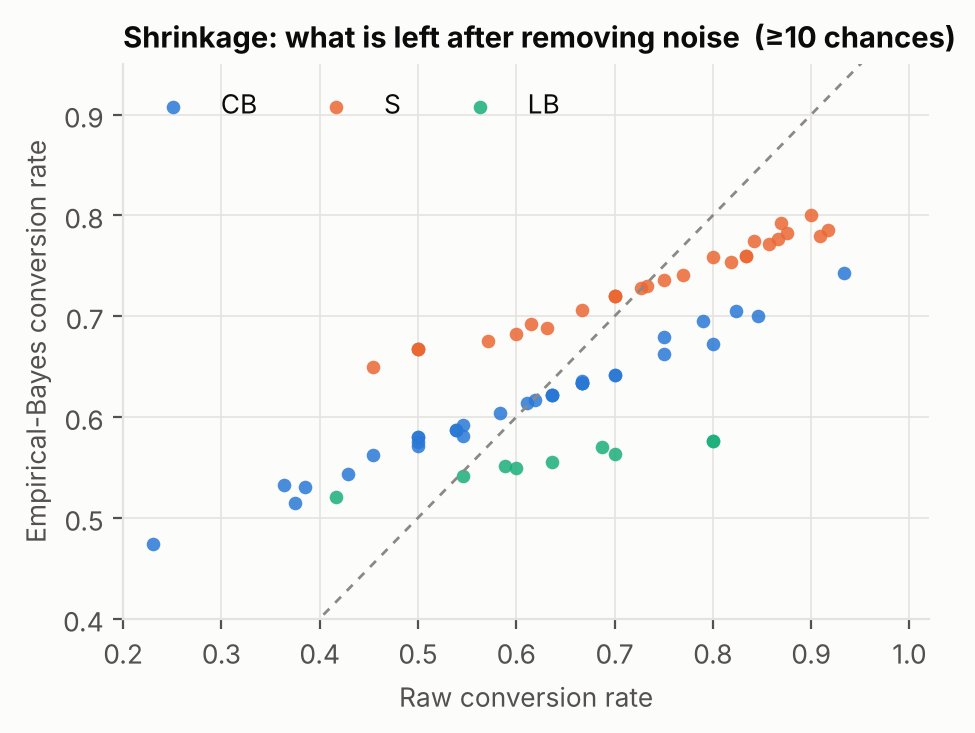
\includegraphics[width=0.62\linewidth]{fig9_shrink.png}
\caption{Raw versus shrunk conversion rates for defenders with at least ten chances.}
\label{fig:shrink}
\end{figure}

\subsection{Leaders}
Figure~\ref{fig:leaders} lists the defenders with the most missed chances since 2022, and Table~\ref{tab:top} gives their raw and shrunk conversion. Shrinkage pulls the worst converters most of the way back toward their position mean. For example, a cornerback who converted 23\% of 13 chances is estimated at 47\% after shrinkage, against a cornerback prior mean of 62\%. At the other end, Table~\ref{tab:eb} lists the best converters with at least twelve chances; all eight are safeties, which mostly reflects the position effect.

\begin{figure}[H]\centering
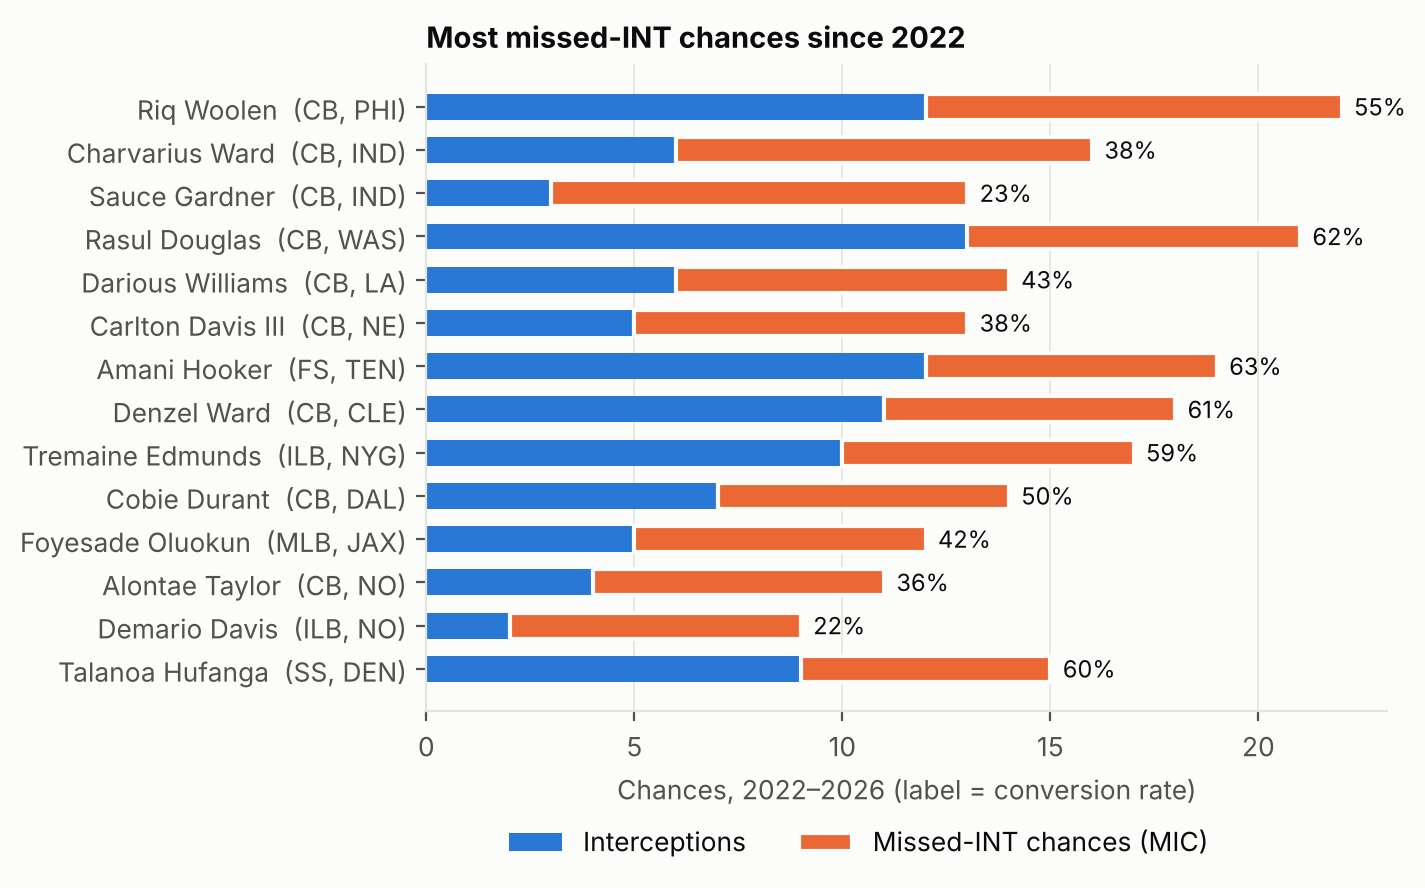
\includegraphics[width=0.86\linewidth]{fig8_leaders.png}
\caption{Defenders with the most missed-INT chances, 2022--2026. Labels show raw conversion.}
\label{fig:leaders}
\end{figure}

\begin{table}[H]\centering\small
\caption{Defenders with the most missed-INT chances, 2022--2026.}\label{tab:top}
\begin{tabular}{llllrrr}\toprule
Defender & Pos. & Team & INT & MIC & Convert & Shrunk \\ \midrule
Charvarius Ward & CB & IND & 6 & 10 & 38\% & 52\% \\
Riq Woolen & CB & PHI & 12 & 10 & 55\% & 58\% \\
Sauce Gardner & CB & IND & 3 & 10 & 23\% & 47\% \\
Darious Williams & CB & LA & 6 & 8 & 43\% & 54\% \\
Rasul Douglas & CB & WAS & 13 & 8 & 62\% & 62\% \\
Carlton Davis III & CB & NE & 5 & 8 & 38\% & 53\% \\
Tremaine Edmunds & ILB & NYG & 10 & 7 & 59\% & 55\% \\
Foyesade Oluokun & MLB & JAX & 5 & 7 & 42\% & 52\% \\
Demario Davis & ILB & NO & 2 & 7 & 22\% & 50\% \\
Amani Hooker & FS & TEN & 12 & 7 & 63\% & 69\% \\
\bottomrule\end{tabular}\end{table}

\begin{table}[H]\centering\small
\caption{Highest shrunk conversion among defenders with at least twelve chances.}\label{tab:eb}
\begin{tabular}{llllrrr}\toprule
Defender & Pos. & Team & INT & MIC & Convert & Shrunk \\ \midrule
Jessie Bates & SS & ATL & 18 & 2 & 90\% & 80\% \\
Kerby Joseph & FS & DET & 20 & 3 & 87\% & 79\% \\
Justin Simmons & FS & ATL & 11 & 1 & 92\% & 78\% \\
Kevin Byard & FS & NE & 14 & 2 & 88\% & 78\% \\
Geno Stone & FS & CIN & 13 & 2 & 87\% & 78\% \\
Xavier McKinney & SS & GB & 16 & 3 & 84\% & 78\% \\
Camryn Bynum & FS & IND & 12 & 2 & 86\% & 77\% \\
Julian Blackmon & FS & NO & 10 & 2 & 83\% & 76\% \\
\bottomrule\end{tabular}\end{table}

\textbf{Face validity.} PFF's public figures name two defenders at opposite ends of the same behavior \cite{pff2024}. In our data the cornerback PFF reports as leading the league in drops has 8 MIC on 14 chances (43\% conversion), and the safety PFF describes as unusually secure has 4 MIC on 15 chances (73\%). The direction agrees; the magnitudes do not and should not, because PFF's windows start in 2020, its drops are judged from film, and ours are an upper-bound proxy.

\subsection{Does counting misses help predict interceptions?}
Table~\ref{tab:pred} and Figure~\ref{fig:pred} show that adding last season's missed chances improves out-of-sample prediction of next season's interceptions. Last-year INT improves on position alone, and Chances improves further. Separating INT from MIC does not help beyond their sum. In the separate-coefficient model an extra pick is associated with 1.19 times as many interceptions next year and an extra miss with 1.13 times, with a ratio of coefficients of 0.7 (95\% CI 0.2 to 1.4). We cannot reject that a miss and a pick are worth the same, and the data are inconsistent with a miss being worth \emph{nothing}.

\begin{figure}[H]\centering
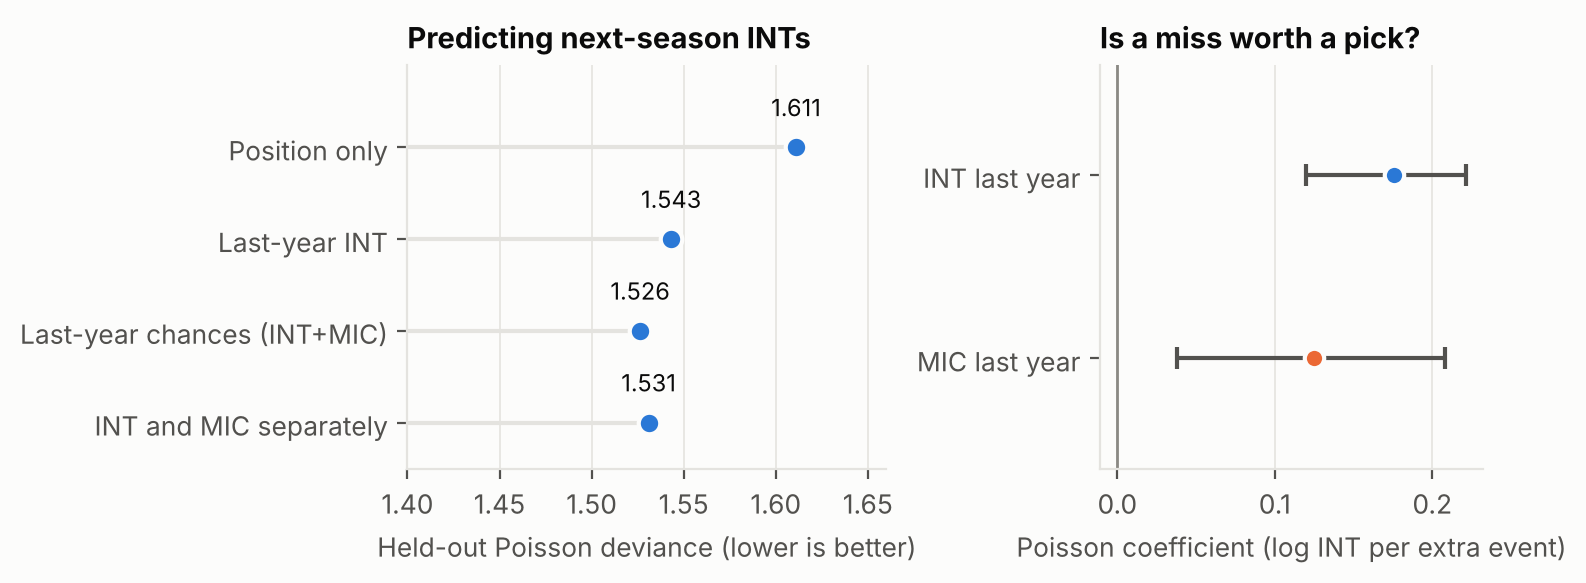
\includegraphics[width=\linewidth]{fig6_prediction.png}
\caption{Left: held-out Poisson deviance for four models of next-season INTs. Right: coefficients with 95\% player-cluster bootstrap intervals.}
\label{fig:pred}
\end{figure}

\begin{table}[H]\centering\small
\caption{Out-of-sample prediction of next-season INTs (leave-one-season-pair-out).}\label{tab:pred}
\begin{tabular}{lrr}\toprule
Model & Held-out deviance & vs.\ position only \\ \midrule
Position only & 1.611 & +0.0\% \\
Last-year INT & 1.543 & -4.2\% \\
Last-year chances (INT+MIC) & 1.526 & -5.3\% \\
INT and MIC separately & 1.531 & -5.0\% \\
\bottomrule\end{tabular}\end{table}

The reading is that MIC carries information about \emph{opportunity}: who is in a position to intercept the ball, through role, scheme and ability to disrupt, and not about hands. A defender with many chances keeps getting them regardless of how the last ones ended.

\subsection{Teams}
At team level there is no persistence at all (Figure~\ref{fig:team}). Season-$t$ team INTs correlate 0.00 with season-$(t{+}1)$ INTs, team Chances correlate -0.03, and the difference in correlation has a 95\% interval of -0.15 to 0.08 across 96 pairs. Team interception totals in this window are best treated as noise, and charting missed chances does not rescue them. Section~\ref{sec:long} repeats this on 26 season pairs and finds a small persistent component.

\begin{figure}[H]\centering
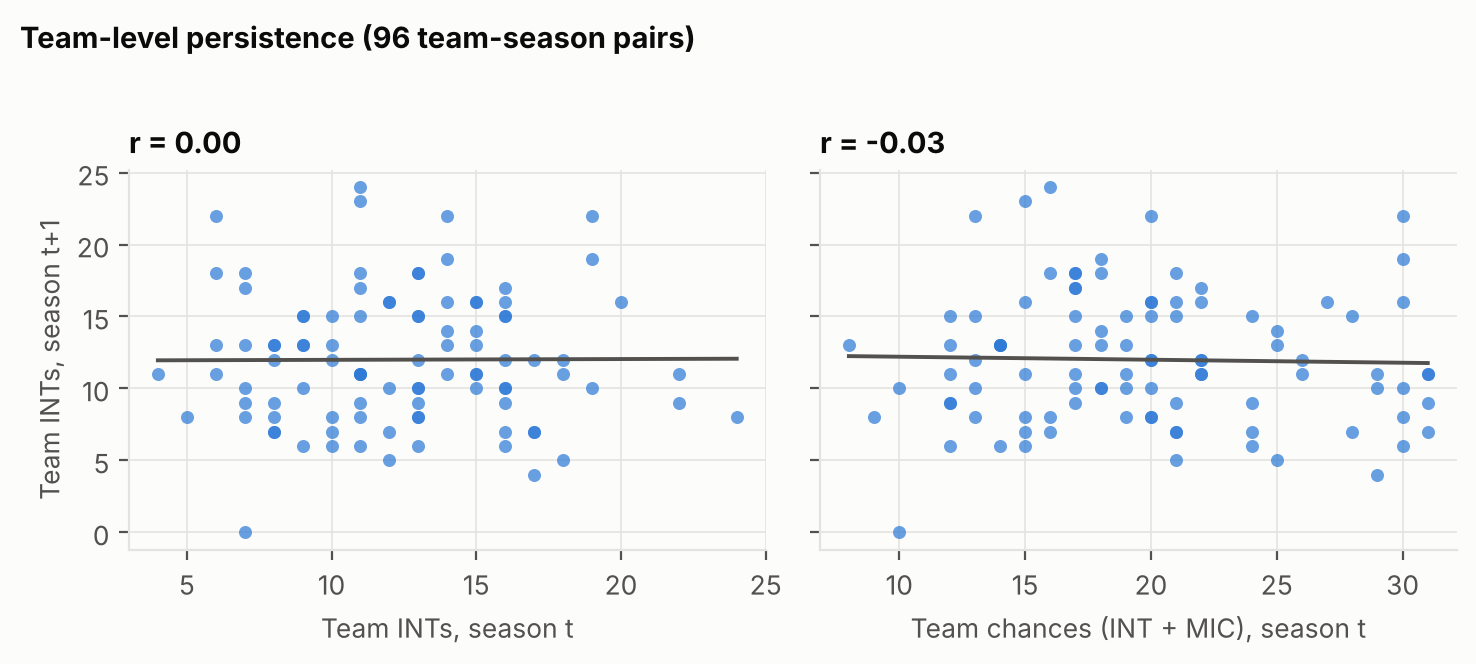
\includegraphics[width=0.92\linewidth]{fig7_team.png}
\caption{Team totals in one season versus team INTs in the next, with least-squares lines.}
\label{fig:team}
\end{figure}

\section{Long-run evidence, 1999--2026}\label{sec:long}
\subsection{Interceptions became rarer; breakups did not}
Figure~\ref{fig:trends} shows what 27 seasons add before any player-level question. Interceptions fell from 3.3\% of pass attempts in 1999--2003 to 2.3\% in 2021--2025, a drop of 30\% (linear trend $p<0.001$), with the lowest season in the window in 2024 at 2.2\%. Passes defended per attempt moved much less, from 9.7\% to 8.7\%. The share of defender plays that end in a catch therefore fell from 24\% to 20\%. Any official statistic, and any leaderboard that compares eras, needs a league baseline for the season it is computed in.

\begin{figure}[H]\centering
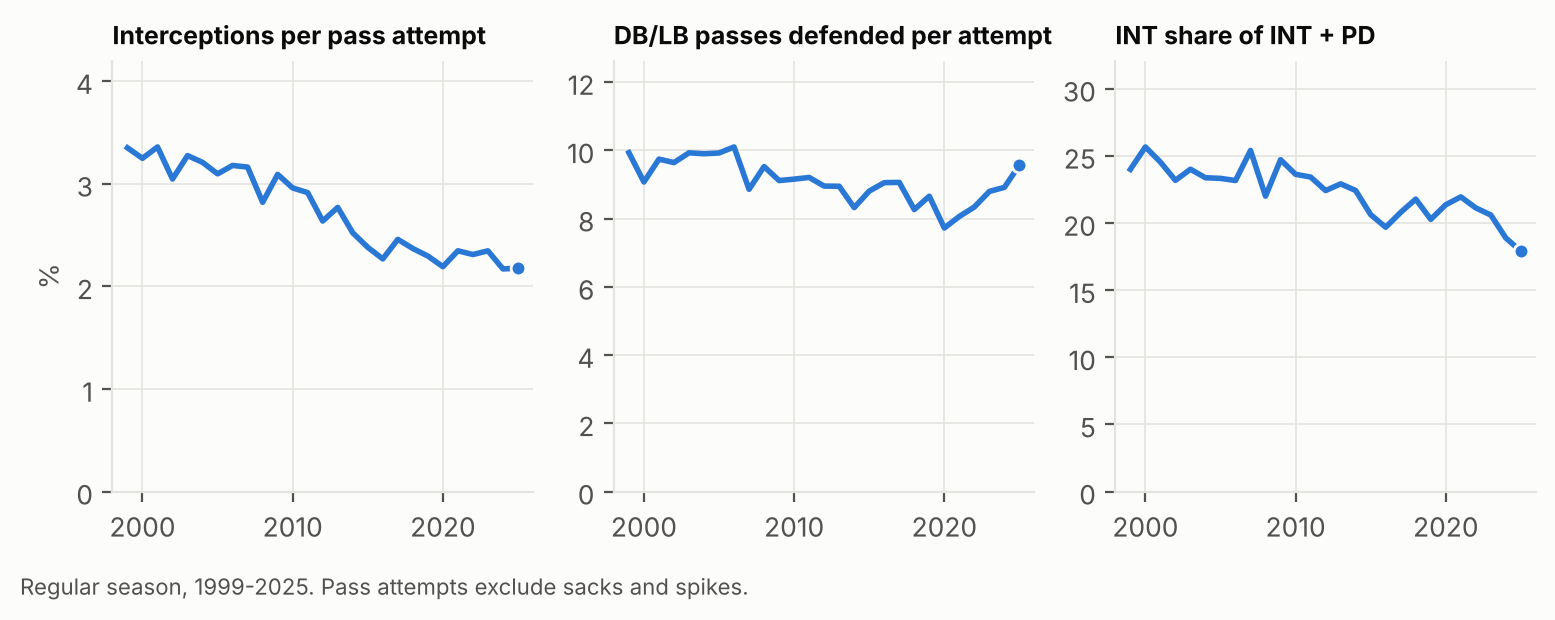
\includegraphics[width=\linewidth]{fig10_trends.png}
\caption{League-wide trends in regular-season interceptions, defensive-back and linebacker passes defended, and the interception share of the two, 1999--2025.}
\label{fig:trends}
\end{figure}

\subsection{Position and era}
Figure~\ref{fig:era} and Table~\ref{tab:era} split INT share by position and seven-year era. Safeties convert about three in ten in every era. Cornerbacks fell from 22\% in 1999--2005 to 17\% in 2020--2025, with intervals that do not overlap between the first two eras and the last two. Linebackers and safeties moved less. The position ordering seen in the charted data (safeties highest) is therefore a long-standing feature and not an artifact of four seasons.

\begin{figure}[H]\centering
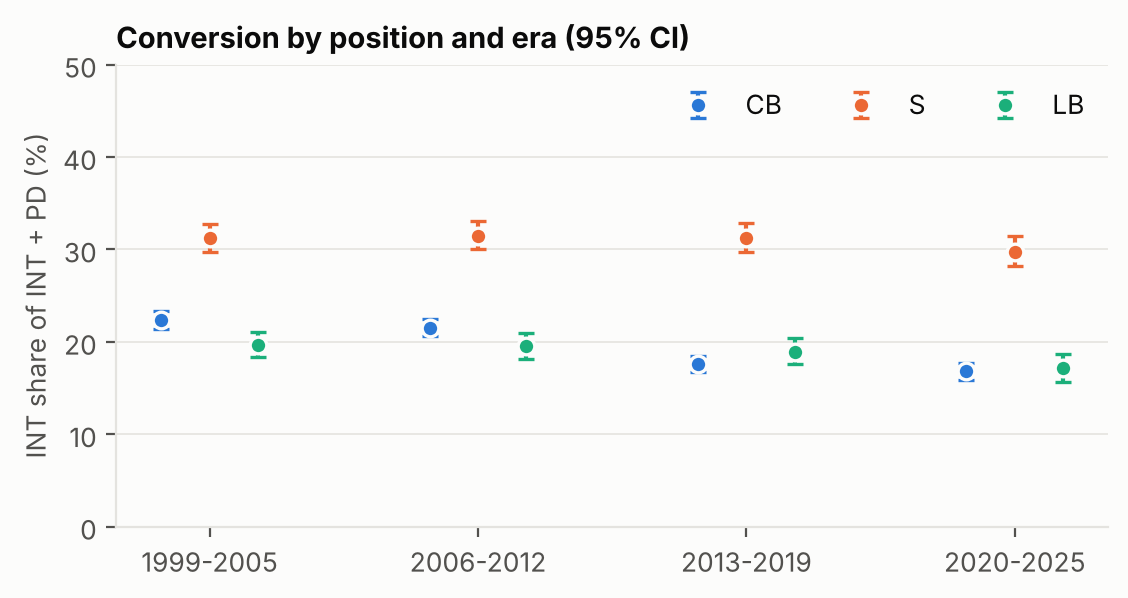
\includegraphics[width=0.78\linewidth]{fig11_position_era.png}
\caption{INT share of INT plus PD by position group and era, with 95\% Wilson intervals.}
\label{fig:era}
\end{figure}

\begin{table}[H]\centering\small
\caption{INT share of INT plus PD by position and era (each cell rests on 2,541 to 7,591 chances).}\label{tab:era}
\begin{tabular}{lrrrr}\toprule
Position & 1999--2005 & 2006--2012 & 2013--2019 & 2020--2025 \\ \midrule
S & 31.3\% & 31.5\% & 31.3\% & 29.8\% \\
CB & 22.3\% & 21.5\% & 17.6\% & 16.8\% \\
LB & 19.6\% & 19.5\% & 18.9\% & 17.1\% \\
\bottomrule\end{tabular}\end{table}

\subsection{Validating PD against charted chances}\label{sec:val}
The 2022--2025 overlap lets us ask how much of PD is MIC. Across 1,131 defender-seasons with both measures, the correlation between PD and MIC counts is 0.37 (95\% CI 0.31 to 0.43), so PD carries information about who is near interception-worthy throws. MIC is only 14\% of PD credits (cornerbacks 12\%, safeties 16\%, linebackers 17\%), which is why INT share is much lower than charted conversion (Figure~\ref{fig:val}). Among the 52 defender-seasons with six or more charted chances, INT share and charted conversion correlate 0.79, but both share the same interception numerator, so that figure is an upper bound on independent agreement. We treat PD as a noisy, diluted measure of opportunity, suitable for relative comparisons across a long window and not for levels.

\begin{figure}[H]\centering
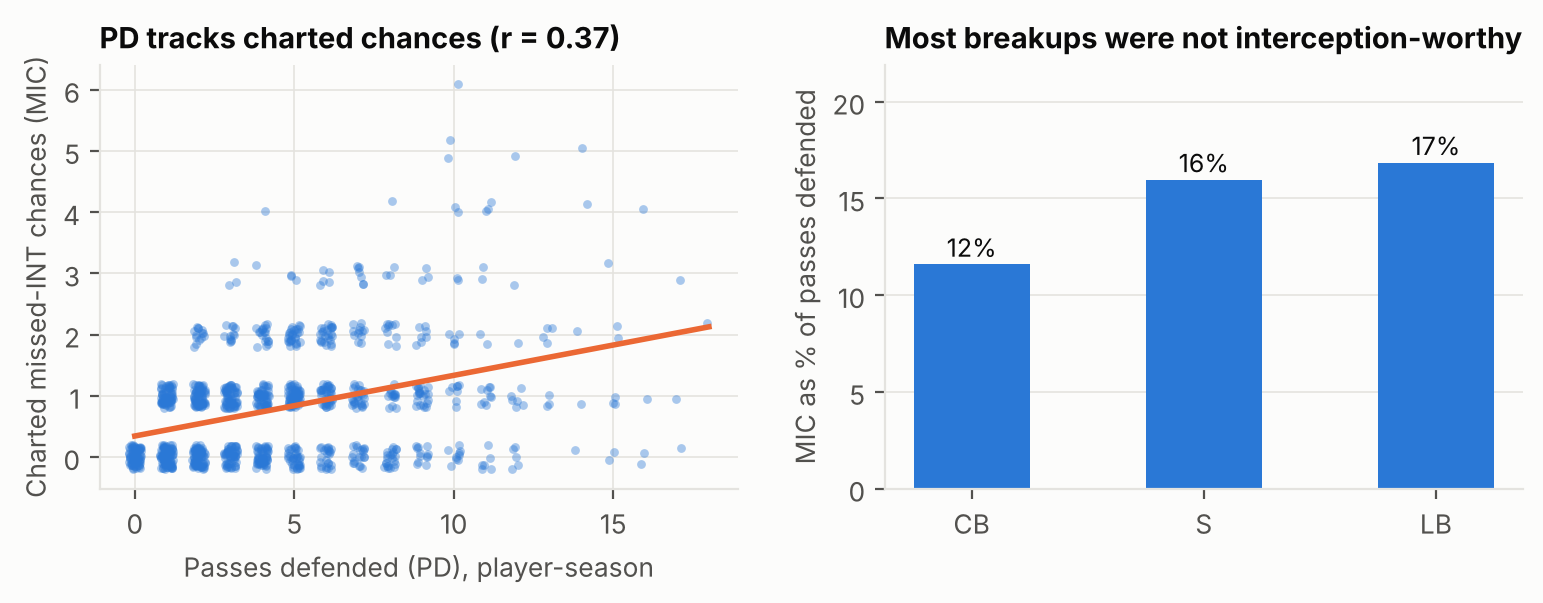
\includegraphics[width=\linewidth]{fig14_validation.png}
\caption{Left: passes defended versus charted missed-INT chances per defender-season, 2022--2025 (points jittered). Right: charted MIC as a share of all passes defended, by position.}
\label{fig:val}
\end{figure}

\subsection{Is conversion a skill? Twenty-seven seasons}
Unlike the four-season charted sample, the long-run data reject pure binomial variation in all three position groups (Table~\ref{tab:lrover}). The fitted true-talent standard deviation of INT share is about 6 points for cornerbacks, 10 for safeties and 8 for linebackers. The signal is real but thin: half reliability needs about 46 chances for cornerbacks, 22 for safeties and 24 for linebackers, against a median of 4 chances per defender-season. Figure~\ref{fig:lrrel} shows the split-half correlations (8 or more chances: cornerbacks 0.06, safeties 0.17, linebackers 0.07) and a year-to-year correlation of 0.16 (95\% CI 0.10 to 0.21, 1,147 pairs).

\begin{table}[H]\centering\small
\caption{Beta-Binomial fits and overdispersion tests for INT share, 1999--2025 (complete player-seasons).}\label{tab:lrover}
\begin{tabular}{lrrrrrrr}\toprule
Position & Player-seasons & Median chances & Prior mean & $\alpha+\beta$ & True-talent SD & LRT & $p$ \\ \midrule
CB & 3,885 & 6 & 19.6\% & 45.8 & 5.8 pts & 59.0 & $<$0.001 \\
S & 2,828 & 4 & 30.8\% & 21.8 & 9.7 pts & 67.8 & $<$0.001 \\
LB & 3,764 & 2 & 18.8\% & 24.1 & 7.8 pts & 34.1 & $<$0.001 \\
\bottomrule\end{tabular}\end{table}

\begin{figure}[H]\centering
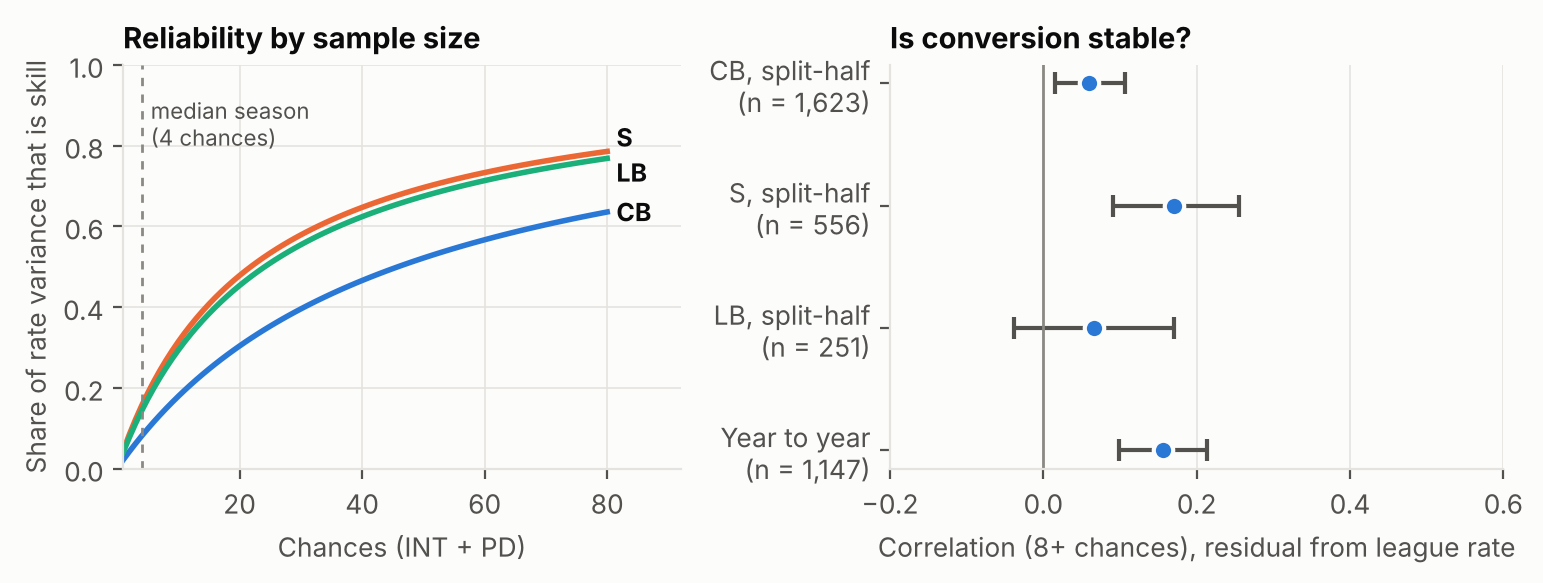
\includegraphics[width=\linewidth]{fig12_longrun_reliability.png}
\caption{Left: reliability of an observed INT share as a function of chances. Right: split-half and year-to-year correlations of INT share, relative to each season's league rate.}
\label{fig:lrrel}
\end{figure}

This is consistent with the charted-era result. A true correlation near 0.15 lies inside the interval we reported for MIC ($-0.05$ to $0.20$), and with about 170 defenders the four-season test has little power to separate 0.15 from zero. The data cannot say whether the persistent component is hands or role: defenders who play more man coverage, line up in the slot, or are targeted differently would also show stable shares.

\subsection{Prediction and teams}
Table~\ref{tab:lrpred} and Figure~\ref{fig:lrpred} repeat the prediction test on 26 season pairs (9,149 defender-pairs). Every model improves on position alone. Chances beat interceptions alone in 22 of 26 held-out seasons, and fitting INT and PD separately does best. The coefficients imply that an extra pass defended is worth about 0.45 of an interception (95\% CI 0.38 to 0.54) for predicting next year's interceptions. In the four charted seasons the same ratio for MIC was 0.7 with a wide interval, so the two estimates are compatible and the longer window pins the number down.

\begin{figure}[H]\centering
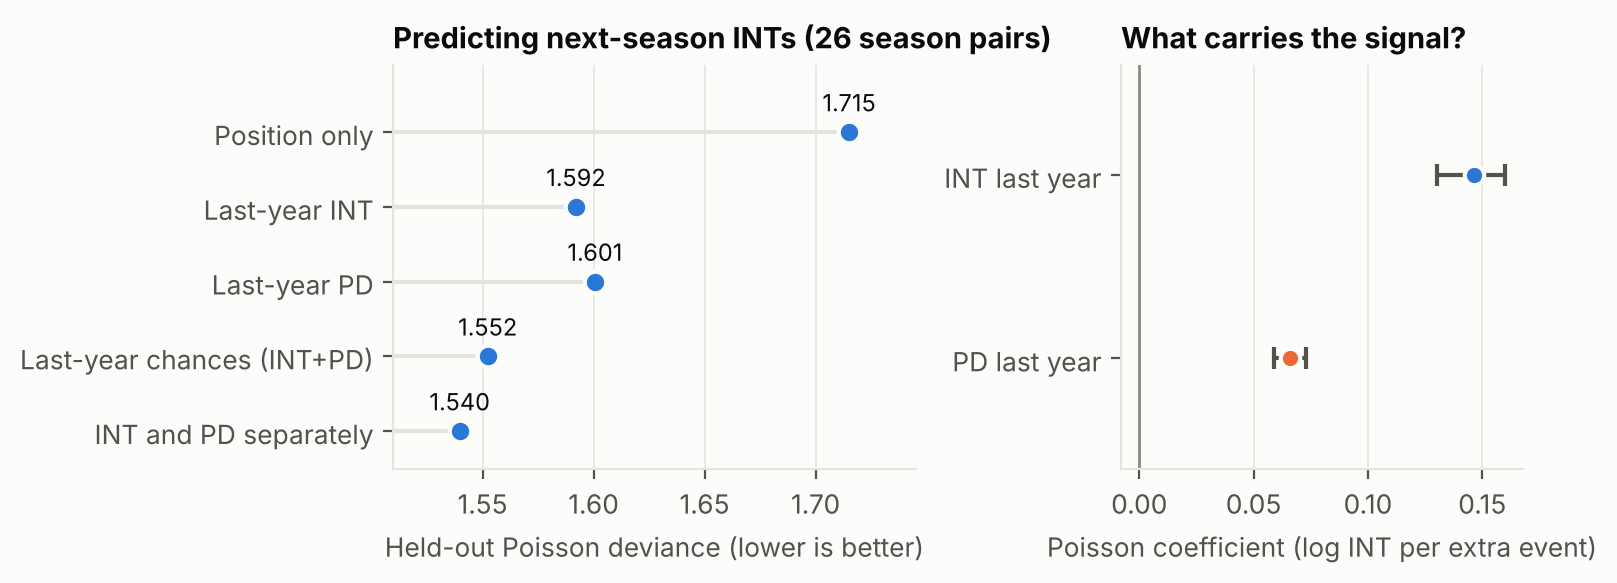
\includegraphics[width=\linewidth]{fig13_longrun_prediction.png}
\caption{Left: held-out deviance for five models of next-season INTs over 26 season pairs. Right: coefficients with 95\% player-cluster bootstrap intervals.}
\label{fig:lrpred}
\end{figure}

\begin{table}[H]\centering\small
\caption{Out-of-sample prediction of next-season INTs, 26 leave-one-season-pair-out folds.}\label{tab:lrpred}
\begin{tabular}{lrrr}\toprule
Model & Held-out deviance & vs.\ position only & Seasons better than INT-only \\ \midrule
Position only & 1.715 & +0.0\% & 0 \\
Last-year INT & 1.592 & -7.2\% & -- \\
Last-year PD & 1.601 & -6.7\% & 11 \\
Last-year chances (INT+PD) & 1.552 & -9.5\% & 22 \\
INT and PD separately & 1.540 & -10.2\% & 25 \\
\bottomrule\end{tabular}\end{table}

At team level, once each season's league mean is removed, team interceptions correlate 0.14 with the next season's (95\% CI 0.08 to 0.22, 829 team-season pairs); team chances correlate 0.13 and team passes defended 0.09. That is small but positive. With only 96 pairs, the charted window's standard error on a correlation is about 0.10, so its null result is not in conflict.

\subsection{Career leaders}
Figure~\ref{fig:lrlead} lists the career interception leaders since 1999 and how many other passes each defended. Shares range from 23\% (Terence Newman) to 50\% (Darren Sharper). Table~\ref{tab:lrhi} and Table~\ref{tab:lrlo} give the highest and lowest shrunk shares among defenders with 80 or more chances. The low end is dominated by cornerbacks with many breakups and few interceptions. Role and scheme can produce that pattern as readily as poor hands, so these tables describe results, not ability.

\begin{figure}[H]\centering
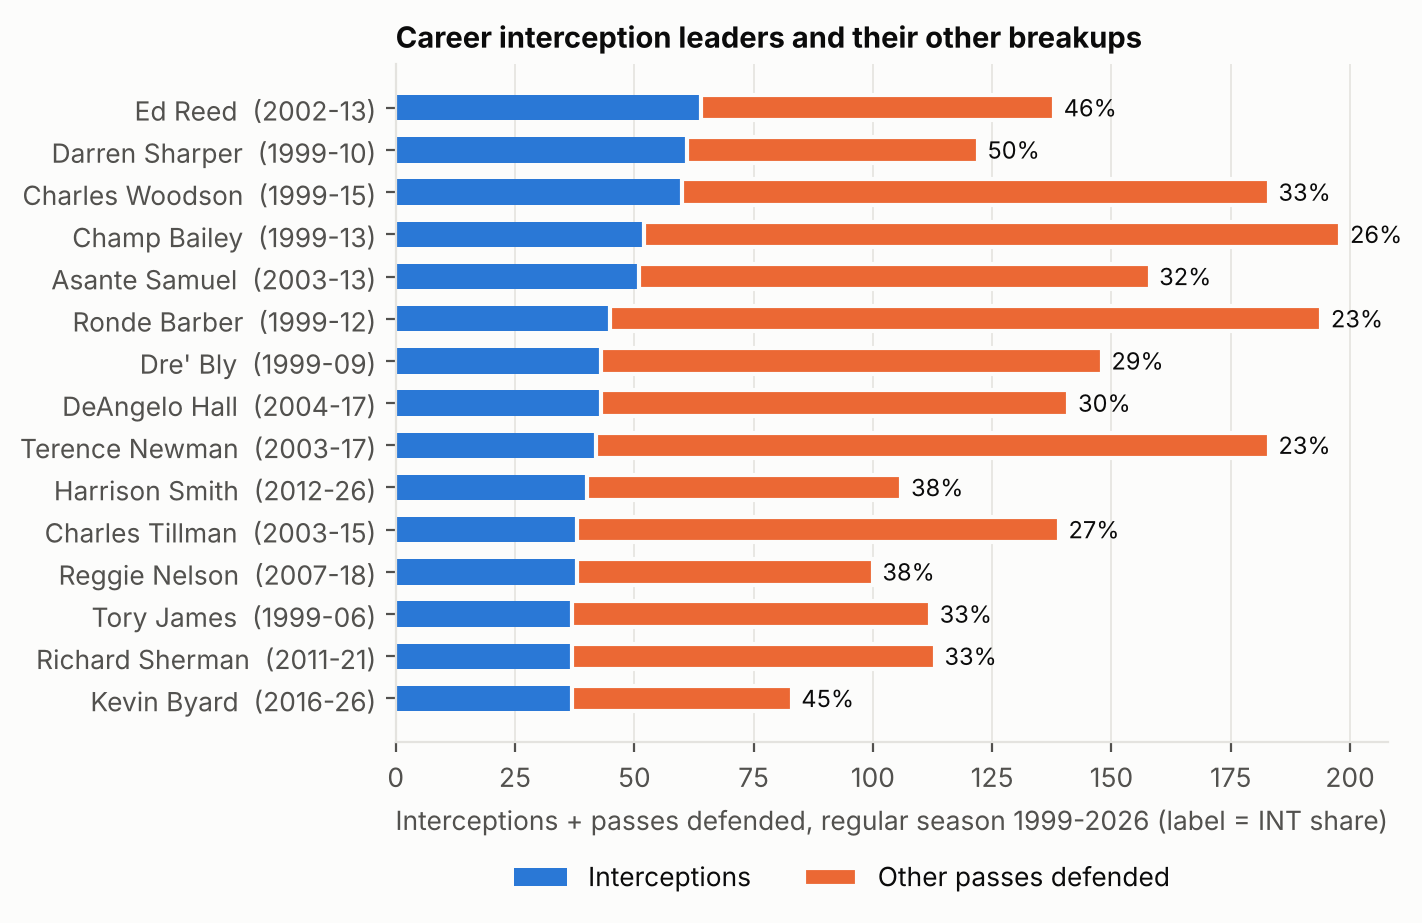
\includegraphics[width=0.86\linewidth]{fig15_longrun_leaders.png}
\caption{Career interception leaders, regular season 1999--2026, with other passes defended. Labels show INT share.}
\label{fig:lrlead}
\end{figure}

\begin{table}[H]\centering\small
\caption{Highest shrunk INT share, defenders with 80 or more chances, 1999--2026.}\label{tab:lrhi}
\begin{tabular}{lllrrrr}\toprule
Defender & Pos. & Years & INT & PD & INT share & Shrunk \\ \midrule
Darren Sharper & FS & 1999--2010 & 61 & 61 & 50\% & 47\% \\
Ed Reed & FS & 2002--2013 & 64 & 74 & 46\% & 44\% \\
Kevin Byard & FS & 2016--2026 & 37 & 46 & 45\% & 42\% \\
Reggie Nelson & FS & 2007--2018 & 38 & 62 & 38\% & 37\% \\
Harrison Smith & FS & 2012--2026 & 40 & 66 & 38\% & 37\% \\
Tyrann Mathieu & FS & 2013--2024 & 36 & 64 & 36\% & 35\% \\
\bottomrule\end{tabular}\end{table}

\begin{table}[H]\centering\small
\caption{Lowest shrunk INT share, defenders with 80 or more chances, 1999--2026.}\label{tab:lrlo}
\begin{tabular}{lllrrrr}\toprule
Defender & Pos. & Years & INT & PD & INT share & Shrunk \\ \midrule
Ronald Darby & CB & 2015--2024 & 8 & 97 & 8\% & 11\% \\
Ivan Taylor & CB & 2003--2014 & 15 & 117 & 11\% & 14\% \\
Buster Skrine & CB & 2011--2021 & 10 & 77 & 12\% & 14\% \\
Carlton Davis III & CB & 2018--2026 & 11 & 81 & 12\% & 14\% \\
Will Allen & CB & 2001--2011 & 15 & 102 & 13\% & 15\% \\
Charvarius Ward & CB & 2018--2026 & 10 & 72 & 12\% & 15\% \\
\bottomrule\end{tabular}\end{table}

\section{What an official statistic should look like}
The evidence supports recording missed chances and argues against ranking individuals by a raw drop rate. Conversion contains a small stable component, so a shrunk rate has some value, but only after many chances. We propose the following.
\begin{enumerate}[nosep]
\item \textbf{Record the event, not the rate.} Add a charted ``dropped interception'' to the official play record, defined as a defender with a clean chance who failed to secure the ball, scored by two independent reviewers with published agreement. Report counts.
\item \textbf{Headline Chances.} Chances (INT plus drops) predicts future interceptions better than INT alone and is the quantity that tracks role and opportunity.
\item \textbf{Publish conversion only with context.} If a rate is shown, show it by position, shrunk toward the position mean, and withhold it below a minimum sample. In the 27-season data a defender needs about 22 chances (safeties) to 46 (cornerbacks) to reach half reliability, and the median defender-season has 4 chances.
\item \textbf{Separate contested from clean.} FTN already records contested-ball and catchability flags; an official chart should keep them so a break-up on a contested throw is not scored as a drop.
\item \textbf{Fix the chart definition.} The drift in Figure~\ref{fig:drift} shows how fragile a charted flag is when its coding instructions change quietly. Any official stat needs a versioned rulebook.
\item \textbf{Publish the era baseline.} The interception rate fell by about 30\% between 1999--2003 and 2021--2025 while breakups per attempt barely moved. A leaderboard should show each season's league rate beside the player's.
\end{enumerate}

\section{Limitations}
\textbf{The proxy is the main limitation.} MIC mixes true drops and legitimate break-ups. Measurement error of that kind attenuates correlations, so the near-zero split-half reliability is a statement about MIC, not necessarily about hands. If film-graded drops were much cleaner than MIC, reliability could be higher than we estimate. The data cannot settle that, and the result should be re-run on PFF-style charted drops if they can be licensed.

\textbf{The long-run measure is looser still.} PD credits include breakups on throws no defender could have caught, depend on official scorers' habits that may have shifted, and say nothing about which throws were catchable. Rosters before 2002 label some defenders only as ``DB''. The long-run results are about relative differences and persistence, and we do not read its levels as drop rates.

\textbf{Charting drift and coverage.} FTN's flag rate falls by about 38\% over the sample, and seasons are not exchangeable in counts.

\textbf{Samples are small.} The median player-season has 2 chances. Four complete seasons give three season-to-season pairs. Intervals are wide and many conclusions are of the form ``cannot be distinguished from luck'', which is weaker than ``is luck''.

\textbf{Attribution.} Pass-defense credits are assigned by official scorers. Roster position uses the depth chart, so an edge rusher listed as OLB is grouped with linebackers. Traded players are assigned to the team where most of their chances occurred. Defensive linemen are excluded (156 interception and pass-defense credits).

\textbf{No coverage denominator.} We do not observe targets in coverage, so Chances is not a rate per snap or per target.

\textbf{Partial 2026.} 2026 (through Week 9) is excluded from the priors, prediction models and team tests, but contributes to career totals, the funnel plots and the split-half test, so those descriptive results are not strictly limited to complete seasons.

\section{Reproducibility}
All code, data and figures are in the project folder. \texttt{build\_dataset.py} downloads the nflverse files and writes the charted CSVs; \texttt{analysis.py} writes the charted figures and \texttt{results.json}; \texttt{build\_longrun.py} and \texttt{analysis\_longrun.py} do the same for 1999--2026 (\texttt{results\_longrun.json}); \texttt{build\_paper.py} regenerates this PDF from both results files; \texttt{build\_dashboard.py} embeds the data in the dashboard. A data dictionary is in the README.

\begin{thebibliography}{9}
\bibitem{swartz2009} C.~Swartz. \emph{10 Statistics That Would Make the NFL Better}. Bleacher Report, 17 March 2009. \url{https://bleacherreport.com/articles/140911-10-statistics-that-would-make-the-nfl-better}
\bibitem{pff2024} Pro Football Focus (undated web articles). \emph{NFL defensive back catch rate, Week 7}. \url{https://www.pff.com/news/nfl-defensive-back-catch-rate-week-7}; see also PFF, \emph{Just how prevalent are dropped interceptions in today's NFL?} \url{https://pff.com/pro-just-how-prevalent-are-dropped-interceptions-in-todays-nfl}
\bibitem{nflverse} nflverse. \emph{nflverse-data releases: play-by-play and rosters}. \url{https://github.com/nflverse/nflverse-data}
\bibitem{ftn} FTN Data via nflverse. \emph{FTN charting data}. See nflverse for license and attribution terms.
\bibitem{efronmorris1975} B.~Efron and C.~Morris. Data analysis using Stein's estimator and its generalizations. \emph{Journal of the American Statistical Association}, 70(350):311--319, 1975.
\bibitem{spiegelhalter2005} D.~J. Spiegelhalter. Funnel plots for comparing institutional performance. \emph{Statistics in Medicine}, 24(8):1185--1202, 2005.
\end{thebibliography}
\end{document}
